\documentclass{beamer}
\usepackage[utf8]{inputenc}
\usepackage[T1]{fontenc}
\usepackage[frenchb]{babel}

\usetheme{Madrid}
\usecolortheme{whale}
\beamertemplatenavigationsymbolsempty

\title{Recalage et fusion de modèles numérisés\\tridimensionnels de grande taille}
\subtitle{MEMO-F-403 - Préparation au mémoire}
\author{Tim Lenertz}
\date{\today}
\institute{ULB}

\maketitle

\begin{document}

\begin{frame}
\frametitle{Introduction}
	\begin{itemize}
	\item \textbf{Nuage de points}\\
		= points sur surface d'objet scanné
	\item Coordonnées dans repère cartésien 3D 
	\item Pris par scanner LIDAR, photogrammétrie
	\item Attribués par couleur RGB, température, intensité, etc.
	\item Pas de connectivité des points
	\item Documentation 3D \\
		(sites archéologiqes, bâtiments, terrain, dent, ...)
	\end{itemize}
\end{frame}

\begin{frame}
\frametitle{Nuage de points - Exemple 1}
	\center
	\includegraphics[width=.8\textwidth]{tower_screenshot.png} \\
	\footnotesize{Modèle de Jacobs University Bremen gGmbH}
\end{frame}

\begin{frame}
\frametitle{Nuage de points - Exemple 2}
	\center
	\includegraphics[width=.9\textwidth]{dragon_screenshot.png} \\
	\footnotesize{Modèle de Stanford Computer Graphics Laboratory}
\end{frame}

\begin{frame}
\frametitle{Scans bruts $\rightarrow$ modèle final}
	\begin{columns}
	\begin{column}[T]{.7\textwidth}
		\begin{itemize}
		\item Planification des scans / photos
		\item Filtrage bruit, outliers
		\item Recalage:
			\begin{itemize}
				\item Mettre plusieurs scans dans même repère
				\item Transformation rigide \\
					(translation, rotation, redimensionnement)
				\item Multiplication matricielle en coordonnées homogènes
				\item Recalage brut (semi-automatisé):
				\item Recalage précis: ICP
			\end{itemize}
		\item Combinaison photo + nuage $\rightarrow$ colorisation
		\item Maillage, feature detection, CAD, ...
		\end{itemize}
	\end{column}
	\begin{column}[T]{.3\textwidth}

	\end{column}
	\end{columns}
\end{frame}

\begin{frame}
\frametitle{Recalage - Exemple 1}
	\center Recalage de 4 scans \footnotesize{\cite{Maka2006}}
	\vspace{5mm}
	\begin{columns}
	\begin{column}[T]{.5\textwidth}
		\includegraphics[height=4cm]{pre_reg.png}
		\center \Large{Avant}
	\end{column}
	\begin{column}[T]{.5\textwidth}
		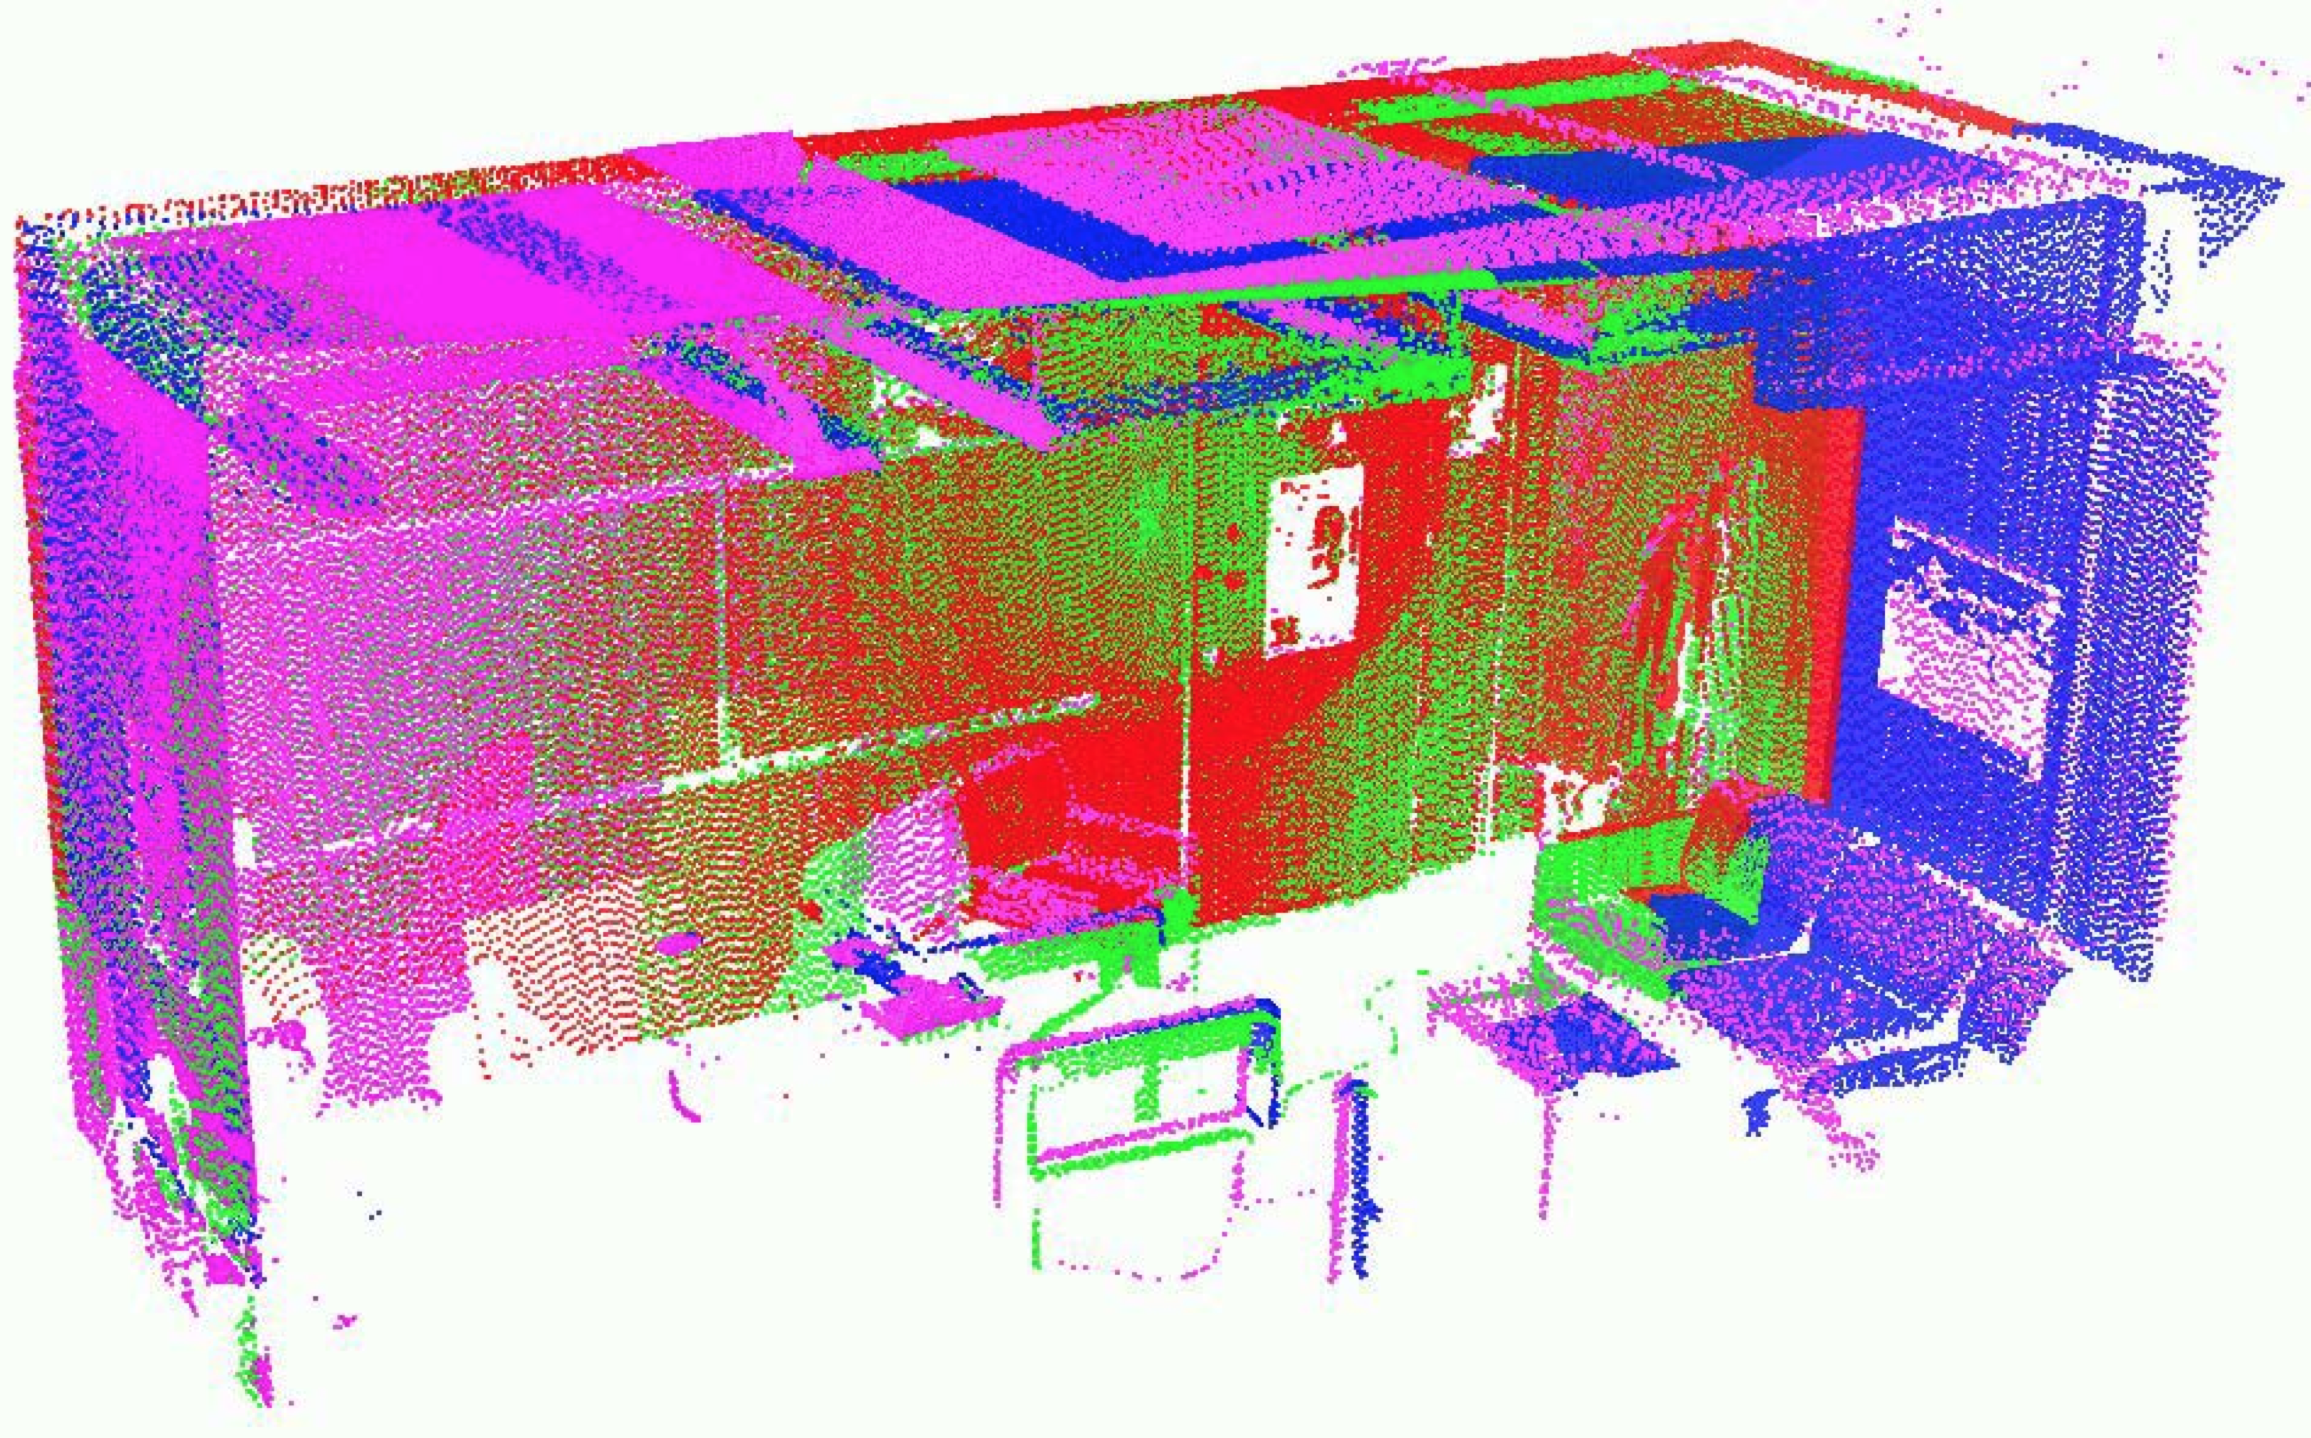
\includegraphics[height=4cm]{post_reg.png}
		\center \Large{Après}
	\end{column}
	\end{columns}
\end{frame}

\begin{frame}
\frametitle{Recalage - Exemple 2}
	\center Recalage de 2 scans { \footnotesize \cite{Mati2011} }
		\\ avec overlap partiel
	\vspace{5mm}
	\begin{columns}
	\begin{column}[T]{.6\textwidth}
		\includegraphics[height=5cm]{pre_reg2.png}
		\center \Large{Avant}
	\end{column}
	\begin{column}[T]{.3\textwidth}
		\includegraphics[height=5cm]{post_reg2.png}
		\center \Large{Après}
	\end{column}
	\end{columns}
\end{frame}

\begin{frame}
\frametitle{Projet de mémoire}
	\begin{itemize}
	\item Recalage et fusion
		\\ scans à grande distance + scans de détails
	\item Densité faible du modèle complet
	\item Grands nombres de points $\rightarrow$ algorithmes efficaces
	\item Développer méthode/algorithmes, établir workflow nécessaire
		\\ i.e. types de scans, photos requis
	\item Scan Hôtel de Ville
	\end{itemize}
	\begin{columns}
		\begin{column}[T]{.5\textwidth}
			\includegraphics[width=\textwidth]{HotelDeVille_08.png}
			\center \Large{Détail}
		\end{column}
		\begin{column}[T]{.5\textwidth}
			\includegraphics[width=\textwidth]{HotelDeVille_06rect.png}
			\center \Large{Modèle complet}
		\end{column}
	\end{columns}
\end{frame}

\begin{frame}
\frametitle{Projet de mémoire}
	\begin{itemize}
	
	\end{itemize}
\end{frame}

\begin{frame}
\frametitle{ICP}
	\begin{itemize}
	\item Iterative Closest Point
	\item Algorithme standard pour recalage précis
	\item Nuages de points \emph{source} et \emph{cible} déjà approximativement alignés
	\item Raffiner itérativement transformation
	\item $\rightarrow$ Minimiser métrique d'erreur
	\end{itemize}
\end{frame}


\bibliographystyle{plain}
\bibliography{../references}

\end{document}
